\chapter{Research methodology}
\label{ch:res_metho}
\rrot{Define research questions}
\rroi{Discuss main research question}
\rroi{Define research boundaries}
\rrod{Define project goals}

Many variations in myocardial perfusion work flow can (significantly) influence the outcome and in turn have consequences for patient treatment. These variation and the relatively new digital SPECT scanners must be validated. 

\section{Project goal}
The goal of the project is to develop a prototype myocardial phantom for dynamic SPECT capable of repeated simulations in typical and cardiac defects situations using  clinical software commonly used in myocardial perfusion scans to ensure compatibility. Most software packages require anatomical recognition points which imposes anatomical requirements on the phantom. In addition, the phantom can be used for educational and training purposes to demonstrate the impact of (poorly) chosen variables, e.g. pressure or flow, scanning parameters, cardiac defects, and so forth.
\subsection{General concept}
\begin{figure}[b!]
	\begin{center}
		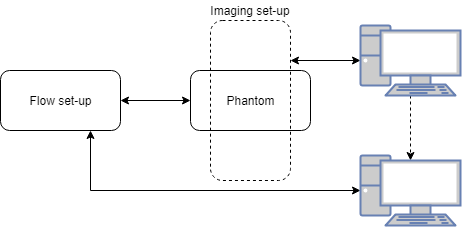
\includegraphics[width=0.75\linewidth]{images/global_setup.png}
	\end{center}
	\caption{General concept, schematic}
	\label{fig:general_concept}
\end{figure}
A general concept is shown in figure \ref{fig:general_concept}. Three main parts can be identified: flow set-up, phantom, and imaging device. The flow set-up consists of everything to produce and maintain pressures and/or flows and measure these variables. The user-interface is a computer or laptop. The phantom consist of everything needed to mimic cardiac defects and to provide a representative image for myocardial perfusion image processing software. The imaging set-up consists of the imaging device itself along with any contrast agents needed to properly image the phantom. Many imaging devices communicate with a dedicated workstation on which the image processing software runs.

\section{Additional resources}
During the individual project of Gijs de Vries, a prototype flow set-up, control module, and calibration set-up has been realised and can be used / re-cycled.
\subsection{Flow set-up}
The flow set-up uses simple, low costs pumps and available flow sensors. These might not be suitable for high precision flow systems. It is encouraged to look into alternatives.
\subsection{Control module}
The control module requires improvement when it is to be re-used. Two of the main improvements consist of improving the electro(magnetic) shielding to decrease the susceptibility to noise and to optimise the pump controllers.
\subsection{Calibration set-up}
The calibration set-up has been shown that it can be used to calibrate flow sensors. Pressure sensors have not been implemented. To increase the precision of the sensors, that are used in the flow set-up or, if decided upon, in a newly developed flow-set-up, the calibration set-up must be made more reliable. It relies too much on human interaction.